%!TEX root = main.tex
\begin{figure}
    \centering
    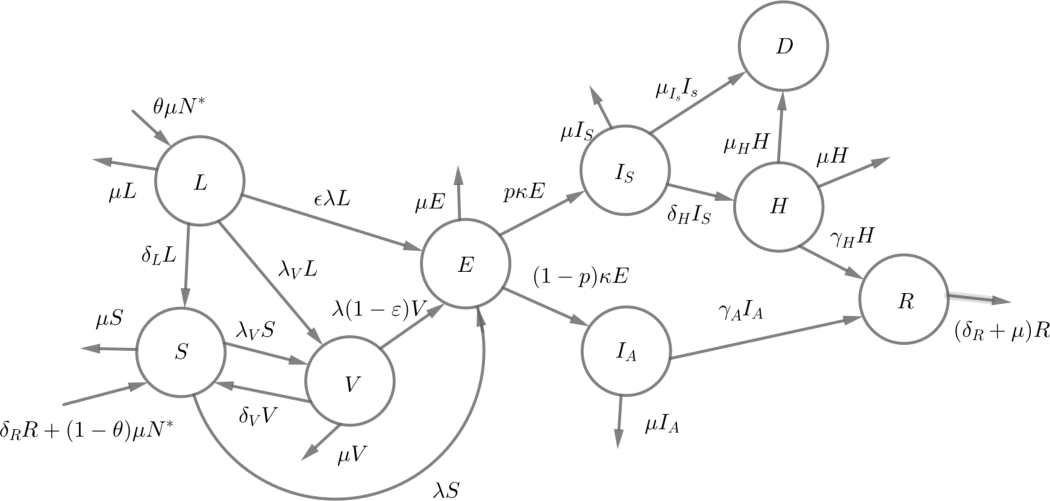
\includegraphics[width=0.7\linewidth]{Figures/Diagrma_Vaccination}
    \caption{Flux diagram for lockdown-vaccination COVID-19 dynamics.}
    \label{fig:model_flux_diagram}
\end{figure}

The reinfection process on COVID-19
disease at the date of writing this manuscript remains under development.
However, our simulations assume reinfection as possible. Thus,
$1/\delta_R$ denote the period of natural immunity. Also we assume that
the underlying vaccine induces immunity that last \num{2}{years}. Furhter, we
take vaccine parameters conforming to Pfizer-BioNTech and Aztra-Zeneca
developments. Above other important modeling assumptions.

\begin{assumptions}
     According to COVID-19 dynamics in model in \Cref{eqn:base_dynamics}, we
     made the following modeling hypotheses about the regarding vaccine.
     \begin{enumerate}[(VH-1)]
        \item
            Vaccine is preventive and only reduce susceptibility.
%            \comment[id=SDIV]{Justify this hypothesis cite}
        \item
            The vaccination camping omits testing to detect seroprevalence.
            Thus Exposed, Infected Asymptomatic and Recovered Asymptomatic
            individuals are undetected but would obtain a vaccine dose
            \textemdash which in these model represent a waste of resources
        \item
            Individuals under Lockdown also would be vaccinated
        \item
            The vaccine is leaky and with efficacy $\epsilon \in[0.7, .975]$
        \item
            Vaccine induced immunity last \SI{2}{years}
        \item
            Natural immunity last a period of \SI{180}{days}
     \end{enumerate}
\end{assumptions}

According to the spread COVID19 dynamics in \Cref{eqn:base_dynamics}, we add
the compartments $L$ and $V$ to denote the Lockdown and Vaccinated population
fractions. Thus, we understand the lockdown intervention as flux between the
Lockdown and Susceptible compartmental with rate $\delta_L$. Because around
\SI{30}{\percent} of the population under risk enclose the children and
young  with scholar age, we assume that a fraction of the susceptible
population in \Cref{eqn:base_dynamics} is under lockdown but in constant flux
with susceptible compartment thus, we formulate the  equations
\begin{equation*}
    \begin{aligned}
        L' =&  \theta \mu N^{\star}
            -(\epsilon \lambda + \delta_L + \lambda_V +\mu) L
        \\
        S' =&
            (1 - \theta) \mu N^\star
            + \delta_L L
            + \delta_V V
            + \delta_R R
        \\
        &-
            \left(
                \lambda + \lambda_V + \mu
            \right) S.
    \end{aligned}
\end{equation*}
%
Since our formulation considers a preventive leaky vaccine we add an output
from lockdown and susceptible compartments by vaccination with rate $\lambda_V$
and add the equation
$$
        V' = \lambda_V  (S + L)
    - \left[
        (1 - \varepsilon) \lambda
        + \delta_V
        + \mu
        \right ] V.
$$
to describe the dynamics of fraction vaccinated population.
Also we add the equations
\begin{equation*}
    \begin{aligned}
        \frac{dX_{vac}}{dt}
            &=
            (u_V(t) + \lambda_V)
            \left[
                L + S + E + I_A + R
            \right]
        \\
        \frac{d Y_{I_S}}{dt}
                & = p \kappa E
    \end{aligned}
\end{equation*}
to account the vaccine coverage and incidence.

Then we establish
the following ordinary differential equation see \Cref{fig:model_flux_diagram}
and \Cref{tbl:dynamics_base_parameters}.
\begin{equation}
    \label{eqn:vacination_dynamics}
    \begin{aligned}
        L' =&  \theta \mu N^{\star}
                -(\epsilon \lambda + \delta_L + \lambda_V +\mu) L
        \\
        S' =&
            (1 - \theta) \mu N^\star
            + \delta_L L
            + \delta_V V
            + \delta_R R
            \\
            &-
            \left(
                \lambda + \lambda_V + \mu
            \right) S
        \\
        E' =&
                \lambda (\epsilon L + (1-\varepsilon) V + S)
                - (\kappa + \mu) E
        \\
        I_S' =&
            p \kappa E
            -
            (
                \delta_H +
                \gamma_S +
                \mu_{I_S} +
                \mu
            ) I_S
        \\
        I_A' = &
                (1 - p) \kappa E - (\gamma_A + \mu) I_A
        \\
        H' = &
            \delta_H I_S - (\gamma_H + \mu_H + \mu) H
        \\
        R' = &
            \gamma_S I_S +
            \gamma_A I_A +
            \gamma_H H
                - (\delta_R + \mu) R
        \\
        D'  = &
                \mu_{I_S} I_S + \mu_H H
        \\
        V' = &
            \lambda_V  (S + L)
            - \left[
                (1 - \varepsilon) \lambda
                + \delta_V
                + \mu
            \right ] V
        \\
        \\
            \frac{dX_{vac}}{dt}
                &=
                (u_V(t) + \lambda_V)
                \left[
                    L + S + E + I_A + R
                \right]
        \\
            \frac{d Y_{I_S}}{dt}
                & = p \kappa E
        \\
            \lambda &:=
                \frac{\beta_A I_A + \beta_S I_S}{N^{\star}}
        \\
        \\
            L(0) &= L_0,
            \ S(0) = S_0,
            \ E(0) = E_0,
        \\
            I_S(0) &= I_{S_{0}},
            I_A(0) = I_{A_{0}},
            H(0) = H_0,
        \\
            R(0) &= R_0, \ D(0) = D_0,
      \\
            V(0) &= 0, \ X_{vac}(0) = 0, \quad
      \\
            X_{vac}(T) &= x_{coverage},
      \\
            N^{\star}(t) &=
                L + S +E + I_S + I_A +
                H + R + V .
        \end{aligned}
\end{equation}